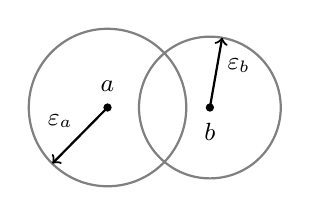
\begin{tikzpicture}[line width=0.8pt, every node/.style={font=\small}]
  \draw[gray] (0,0) circle (1);
  \draw[gray] (1.3,0) circle (0.9);
  \fill (0,0) circle (1.5pt) node[above=2pt] {$a$};
  \fill (1.3,0) circle (1.5pt) node[below=2pt] {$b$};
  \draw[->] (0,0) -- node[pos=0.5, above left=-1pt] {$\varepsilon_a$} (-0.7,-0.71);
  \draw[->] (1.3,0) -- node[pos=0.6, right] {$\varepsilon_b$} (1.456,0.886);
\end{tikzpicture}
